\documentclass{article}
\usepackage{CJKutf8}
\usepackage{geometry,booktabs,pgfplots,listings}
\pgfplotsset{compat=1.18}
\geometry{left=2.5cm,right=2cm,top=2.5cm,bottom=2.5cm}
\lstset{language=C,basicstyle=\ttfamily\small,numbers=left,frame=single,breaklines=true}
\begin{document}\begin{CJK*}{UTF8}{gbsn}
\title{Search Tree Performance Comparison\\BST and Splay Tree}
\author{Group number: \underline{\hspace{3cm}}}\date{\today}\maketitle
\begin{abstract}
本实验实现并比较非平衡二叉搜索树（BST）和伸展树（Splay Tree）的插入、删除与查找。测试包括递增插入递增删除、递增插入逆序删除、随机插入随机删除三种序列。结果显示，BST 在有序数据下退化为链，而 Splay Tree 通过伸展操作保持良好的摊还性能。
\end{abstract}
\section{Introduction}
BST 维护左子树键值小于根、右子树键值大于根的性质。普通 BST 不主动调整树高，有序插入时可能退化为高度为 $N$ 的链。Splay Tree 在每次访问后将目标节点（或最后访问节点）伸展到根，单次最坏复杂度为 $O(N)$，但任意序列的摊还复杂度为 $O(\log N)$。本报告只讨论这两种结构，所有键值互不相同。
\section{Data Structure and Algorithm Specification}
\subsection{BST}
节点由整数键值和两个子指针组成。插入从根递归下降，空指针处创建节点；重复键忽略。查找沿比较结果下降。删除分为叶节点、单子节点和双子节点三种情况；双子节点使用右子树最小节点（中序后继）替换后递归删除。
\begin{lstlisting}
TreeNode *DeleteNode(TreeNode *Root, int val) {
    if (Root == NULL) return NULL;
    if (val < Root->val) Root->Left = DeleteNode(Root->Left, val);
    else if (val > Root->val) Root->Right = DeleteNode(Root->Right, val);
    else if (Root->Left == NULL) { TreeNode *p=Root->Right; free(Root); return p; }
    else if (Root->Right == NULL) { TreeNode *p=Root->Left; free(Root); return p; }
    else { TreeNode *p=GetMin(Root->Right); Root->val=p->val;
           Root->Right=DeleteNode(Root->Right,p->val); }
    return Root;
}
\end{lstlisting}
\subsection{Splay Tree}
Splay 使用 top-down 算法。临时头结点把访问路径拆为左、中、右三部分，循环执行 zig-zig 和链接，最后重新拼接。插入先伸展目标键，再把新节点置于根；删除先伸展目标，若存在则将左子树最大节点伸展到根并接回原右子树。
\begin{lstlisting}
SplayTree *Splay_Delete(SplayTree *Root, int val) {
    if (Root == NULL) return NULL; Root=Splay(Root,val);
    if (Root->val != val) return Root;
    SplayTree *old=Root, *right;
    if (Root->Left == NULL) Root=Root->Right;
    else { right=Root->Right; Root=Splay(Root->Left,val); Root->Right=right; }
    free(old); return Root;
}
\end{lstlisting}
\section{Testing Results}
\subsection{Test design}
\texttt{test.c} 先验证插入、查找、删除和删除后的集合内容，然后执行三种性能实验：Case 1 递增插入递增删除；Case 2 递增插入逆序删除；Case 3 随机插入随机删除。随机序列使用固定种子 $114514$。当前代码实际接受 $1000\leq N\leq20000$，提示中的 $100000$ 上限需要后续统一。
\begin{table}[ht]\centering\caption{平均运行时间（秒）}\label{tab:runtime}
\begin{tabular}{crrrrrr}\toprule
$N$&\multicolumn{2}{c}{Case 1}&\multicolumn{2}{c}{Case 2}&\multicolumn{2}{c}{Case 3}\\
&BST&Splay&BST&Splay&BST&Splay\\\midrule
1000&0.005&0.000&0.007&0.000&0.000&0.000\\
5000&0.105&0.000&0.209&0.001&0.001&0.001\\
10000&0.374&0.001&0.789&0.001&0.002&0.002\\
20000&1.641&0.001&3.303&0.000&0.005&0.005\\\bottomrule
\end{tabular}\end{table}
\begin{figure}[ht]\centering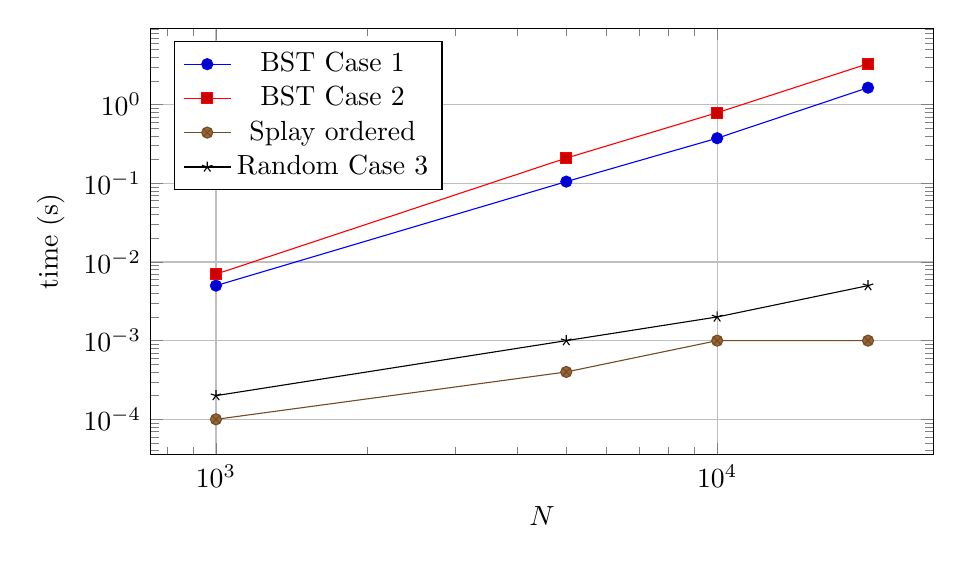
\begin{tikzpicture}
\begin{axis}[width=.95\linewidth,height=7cm,xmode=log,ymode=log,grid=major,xlabel={$N$},ylabel={time (s)},legend pos=north west]
\addplot coordinates{(1000,.005)(5000,.105)(10000,.374)(20000,1.641)};\addlegendentry{BST Case 1}
\addplot coordinates{(1000,.007)(5000,.209)(10000,.789)(20000,3.303)};\addlegendentry{BST Case 2}
\addplot coordinates{(1000,.0001)(5000,.0004)(10000,.001)(20000,.001)};\addlegendentry{Splay ordered}
\addplot coordinates{(1000,.0002)(5000,.001)(10000,.002)(20000,.005)};\addlegendentry{Random Case 3}
\end{axis}\end{tikzpicture}\caption{运行时间趋势。零值计时点以小占位值绘图，表格保留原始输出。}\end{figure}
\section{Analysis and Comments}
BST 的操作复杂度为 $O(h)$。随机输入时树高通常为 $O(\log N)$；有序插入时 $h=O(N)$，因此 Case 1 和 Case 2 呈近似二次增长，逆序删除的遍历代价更大。Splay 单次操作最坏为 $O(N)$，但摊还为 $O(\log N)$，有序场景中访问局部性使其明显优于退化 BST；随机场景下两者性能接近。Splay 不保存平衡因子，代价是树形随访问序列改变。
\texttt{clock()} 的分辨率有限，表中 $0.000$ 不表示真实耗时为零。更严格的实验应提高精度、统一 $N$ 上限并重复测量取平均。
\section{Conclusion}
本实验完成了 BST 和 Splay Tree 的结构、插入、查找和删除。实验验证了普通 BST 对有序输入敏感，而 Splay Tree 对有序访问更稳定；随机输入下 BST 实现更简单，Splay 则具有自适应优势。
\section{Author list}BST implementation, Splay implementation, testing, and report: \underline{\hspace{5cm}}.
\appendix\section{Source Code Interface}实现位于项目根目录的 \texttt{main.c}，实验驱动位于 \texttt{test.c}；本报告未修改二者。
\end{CJK*}\end{document}
